%!TeX spellcheck = en-GB

%Basics
\documentclass[aps, prb, a4paper, english, 12pt, onecolumn, longbibliography, amsmath, amssymb, colorinlistoftodos, floatfix, svgnames]{revtex4-2}
\usepackage[utf8]{inputenc}
\usepackage{babel}

%Symbols and scientifics
\usepackage{amsmath, amsfonts, amssymb, bm}
\numberwithin{equation}{subsection}
\usepackage{physics}
\usepackage{mathtools}
\usepackage{siunitx}
\sisetup{
	per-mode = power ,
	round-mode = figures ,
	round-precision = 3 ,
	scientific-notation = false ,
	output-decimal-marker = {.} ,
	exponent-product = \times ,
	separate-uncertainty = true ,
	uncertainty-separator = \ ,
	output-product = \cdot ,
	quotient-mode = fraction ,
	range-phrase = - ,
	range-units =  single ,
	inter-unit-product = \ensuremath{{\cdot{}}} ,
	number-unit-product = \ ,
	multi-part-units = single ,
	alsoload = synchem ,
	alsoload = addn
}
\DeclareSIUnit\atm{atm}
\usepackage{chemfig}
\usepackage{tikzorbital}

%Appendix, TOC and Bibliography
\usepackage{appendix}
\renewcommand\appendixtocname{Appendices}
%\usepackage[nottoc]{tocbibind}
\usepackage[lastpage,user]{zref}

%Figures
\usepackage{float}
\usepackage{xcolor} % Required to specify font color
\usepackage{graphicx}
\usepackage{subcaption}
\usepackage[format=plain,
            labelfont={bf,it},
            textfont=it]{caption}
\usepackage[verbose]{wrapfig}
\usepackage[a4paper, centering, rmargin=2.5cm, tmargin=2.5cm, lmargin=2.5cm, bmargin=2.5cm]{geometry}
\usepackage{etoolbox}
\usepackage{verbatim}
\usepackage[space]{grffile}
\usepackage[final]{pdfpages}
\usepackage{array}
\usepackage{multirow}
\usepackage{dcolumn}
%\usepackage{animate}
\usepackage{fontawesome}
\usepackage[european]{circuitikz}
\usepackage{pdflscape}
\usepackage{pgfplots}
\pgfplotsset{width=10cm, compat=newest}
\def\axisdefaultwidth{10cm}
%\usepgfplotslibrary{external}
\usepgfplotslibrary{units}
%\tikzexternalize
\usepackage{pgfgantt}
\newcounter{myWeekNum}
\stepcounter{myWeekNum}
%
\newcommand{\myWeek}{\themyWeekNum
    \stepcounter{myWeekNum}
    \ifnum\themyWeekNum=53
         \setcounter{myWeekNum}{1}
    \else\fi
}
%

%Header footer
\usepackage{fancyhdr}
\pagestyle{fancy}
\lhead{C. V. Sørensen \\ R. K. F. Wiuff}
\chead{Quantum Transport in NPG\\DTU Department of Physics}
\rhead{May \nth{1}\\2019}
\cfoot{Page \thepage\, of \zpageref{LastPage}}
\renewcommand{\headrulewidth}{0.4pt}
\renewcommand{\footrulewidth}{0.4pt}

%Text tools
\usepackage[super]{nth}
\usepackage[normalem]{ulem}
\usepackage{import}
\usepackage{url}
\usepackage{lipsum}
\usepackage{microtype}
\usepackage[pdfencoding=auto, psdextra]{hyperref}
\hypersetup{
	colorlinks   = true, %Colours links instead of ugly boxes
	urlcolor     = blue, %Colour for external hyperlinks
	linkcolor    = blue, %Colour of internal links
	citecolor   = red %Colour of citations
}
\usepackage[capitalise]{cleveref}
\usepackage{enumitem}
\setlist[enumerate]{itemsep=0mm}
\usepackage{booktabs}
\usepackage{silence}
\usepackage{todonotes}
\WarningFilter{revtex4-2}{Repair the float package.}

%Python
\usepackage{minted}
\setminted{fontsize=\small}
\usemintedstyle{monokai}
\renewcommand{\listoflistingscaption}{Listings}
%\renewcommand{\MintedPygmentize}{C:/Users/rwiuf/AppData/Roaming/Python/Python37/Scripts/pygmentize}
\newcommand{\im}[2]{\inputminted[bgcolor=Black,linenos=true]{#1}{#2}}

%Definitions and new commands
\newcommand{\degr}{^{\circ}}
\newcommand{\me}{\mathrm{e}}
\newcommand*\mathinhead[2]{\texorpdfstring{$\boldsymbol{#1}$}{#2}}
%PDFPages and RevTeX incompatability fix
\makeatletter
\AtBeginDocument{\let\LS@rot\@undefined}
\makeatother

\begin{document}
%Titlepage herunder:
\begin{abstract}
	\vspace{5mm}
	\centering
	\begin{description}
		\item[Abstract] Abstract... \vspace{3\baselineskip}
	\end{description}
	
\includegraphics[width=1cm]{Figures/DTU3CMYK.eps}
\end{abstract}

\title{Quantum Transport in Nanoporous Graphene}
\date{May \nth{1} 2019}
\author{Rasmus Kronborg Finnemann Wiuff (s163977)}
\email[E-mail at ]{rwiuff@dtu.dk}
\author{Christoffer Vendelbo Sørensen (163965)}
\email[E-mail at ]{chves@dtu.dk}
\affiliation{Technical University of Denmark}
\homepage[Homepage of the Technical University of Denmark ]{http://www.dtu.dk/english/}
\homepage[\\\faGithub \ Project Repository: ]{https://github.com/rwiuff/QuantumTransport}
\maketitle

\pagenumbering{arabic}
\twocolumngrid
\tableofcontents
\onecolumngrid

% ToC before List-ofs fix
\makeatletter
\let\toc@pre\relax
\let\toc@post\relax
\makeatother

\thispagestyle{empty}
%\newpage
\setcounter{page}{1}

%Text
\section{Introduction}
%!TEX root = ../Main.tex
\lipsum{5}\cite{calogero_electron_2019}
\subsection{Pi-orbitals and Basis sets }
\section{Quantum transport}
%!TEX root = ../Main.tex
In this section, the basics of the tight-binding approximation for electron transport will be explained. This motivates the use of numerical routines using NumPy.
\subsection{Ballistic quantum transport}
As graphene is a two dimensional material that consists of carbon atoms arranged in a hexagonal pattern, features in such a material can approach nanometer and sub nanometer scales. Because of the small scale the electrical properties of the material is vastly different from normal materials. Usually when describing the electrical properties of a material, drift-diffusion current models are used. They describe electric charges per area and current per area. This is usually a good description in systems where electron-electron and electron-atom scatterubg frequently occurs. The distance an electron travels before such a event is called its \textit{mean free path}. However, in small systems as those of NPG-devices, the mean free path is longer than the system itself. Experiments have shown that electrons can move ballistically in graphene and carbon nanotubes[litt], that is, without phonon scattering. Therefore, we model electron transport using the \textit{ballistic model}. In this model the electrons move through the material as waves. The fact that the electrons moves as waves will prove important later on because it gives rise to \textit{Quantum Interference} which can be exploited as a tool when engineering graphene-based devices. Furthermore the model looks at only one electron at a time in the presence of an electron gas. This model has been used with big success for regular graphene and it seems that the ballistic model also gives a good approximation for NPGs.
\subsection{\mathinhead{\pi}{\pi}-orbitals and \mathinhead{\pi}{\pi}-electrons}
When modelling the electron transport in graphene one needs to address the orbital structure of carbon lattices. The orbital structure is exactly what motivate the use of tight binding approximation and Green's functions. The two concepts of Tight-binding approximation and Green's functions will be elaborated further in the coming sections.
In its basic form graphene can be divided into rings of carbon atoms as shown in \cref{ring}. In the (\(x,y\))-plane the carbon atoms are bound in \(sp^2\) orbitals as shown in \cref{sp2}.
\begin{figure}[ht]
    \centering
    \begin{subfigure}[b]{0.3\textwidth}
	    \begin{tikzpicture}
		    \chemfig{C*6(-C-C-C-C-C-)}
	    \end{tikzpicture}
	    \caption{Graphene lattices consists of hexagonal arrangements of carbon atoms.}\label{ring}
    \end{subfigure}
    ~
    \begin{subfigure}[b]{0.3\textwidth}
	\centering
	\resizebox{\textwidth}{!}{
		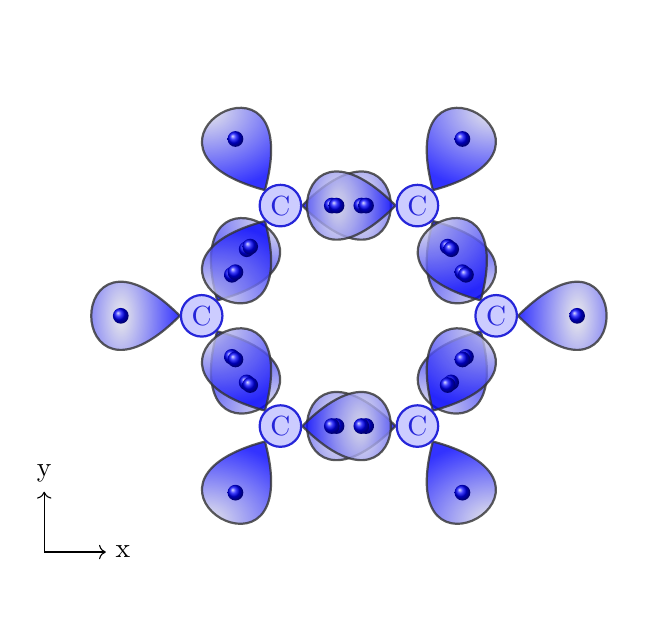
\begin{tikzpicture}
		    \node (x) at (-1,-3) {x};
		    \node (y) at (-2,-2) {y};
		    \draw[->] (-2,-3) -- (x);
		    \draw[->] (-2,-3) -- (y);
			\satom[name=C, color=blue, pos={(0,0)}]{
				blue/60/north east/2/1,
				blue/180/west/1,
				blue/300/south east/2/1
			}
			\satom[name=C, color=blue, pos={(1,1.4)}]{
				blue/0/east/2/1,
				blue/120/north west/1,
				blue/240/south west/2/1
			}
			\satom[name=C, color=blue, pos={(2.74,1.4)}]{
				blue/60/north east/1,
				blue/180/west/2/1,
				blue/300/south east/2/1
			}
			\satom[name=C, color=blue, pos={(3.74,0)}]{
				blue/0/east/1,
				blue/120/north west/2/1,
				blue/240/south west/2/1
			}
			\satom[name=C, color=blue, pos={(2.74,-1.4)}]{
				blue/60/north east/2/1,
				blue/180/west/2/1,
				blue/300/south east/1
			}
			\satom[name=C, color=blue, pos={(1,-1.4)}]{
				blue/0/east/2/1,
				blue/120/north west/2/1,
				blue/240/south west/1
			}
		\end{tikzpicture}}
	\caption{Carbon atoms in a hexagonal lattice are \(sp^2\) hybridised in the (\(x,y\))-plane.}\label{sp2}
    \end{subfigure}
    \caption{Benzene ring and its \(sp^2\) hybradised orbitals.}\label{Benz}
\end{figure}
This hybridisation lock all but one valence electron for the carbon atoms. These electrons exists in a p-orbital in the \(z\)-direction.
\cref{p} shows the valence orbitals of carbon.
\begin{figure}[H]
	\begin{center}
		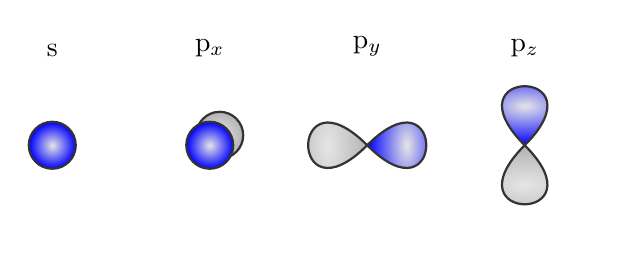
\begin{tikzpicture}
			\orbital[pos = {(0,3)}] {s}
			\node[above] at (0,4) {s};
			\orbital[pos = {(2,3)}]{px}
			\node[above] at (2,4) {p$_x$};
			\orbital[pos = {(4,3)}]{py}
			\node[above] at (4,4) {p$_y$};
			\orbital[pos = {(6,3)}]{pz}
			\node[above] at (6,4) {p$_z$};
		\end{tikzpicture}
		\caption{The valence orbitals of carbon.}
		\label{p}
	\end{center}
\end{figure}
The last electron in the p\(_z\) orbital does not mix with the tightly bound s, p\(_x\) and p\(_y\) electrons and moves freely. Thus these electrons have higher energies compared to the \(sp^2\) electrons and occupy states at the Fermi level. These electrons dominates transport in the graphene lattice. The p\(_z\) orbital is also known as the \(\pi\)-orbital and as such the electron lying there is called a \(\pi\)-electron. Through a carbon lattice the \(\pi\)-electrons will travel through \(\pi\)-orbitals. For a benzene ring the \(\pi\)-electrons at the highest occupied molecular state will travel through the p\(_\pi\)-orbitals switching sign as they travel as shown in \cref{sign}.
\begin{figure}[H]
	\begin{center}
		\pgfdeclarelayer{background}
		\pgfdeclarelayer{middle}
		\pgfdeclarelayer{foreground}
		\pgfsetlayers{background,middle,main,foreground}
		\begin{tikzpicture}
			\begin{pgfonlayer}{background}
				\orbital[pos = {(6,6)}]{-pz}
				\node[above] at (6,7) {-p$_\pi$};
				\orbital[pos = {(4,6)}]{pz}
				\node[above] at (4,7) {p$_\pi$};
				\draw[dashed, very thick] (6,6) -- (4,6);
				\draw[dashed, very thick] (7,4.73) -- (6,6);
				\draw[dashed, very thick] (4,6) -- (3,4.73);
			\end{pgfonlayer}
			\orbital[pos = {(7,4.73)}]{pz}
			\node[above] at (7,5.73) {p$_\pi$};
			\orbital[pos = {(3,4.73)}]{-pz}
			\node[above] at (3,5.73) {-p$_\pi$};
			\begin{pgfonlayer}{foreground}
				\orbital[pos = {(4,3.46)}]{pz}
				\node[above] at (4,4.46) {p$_\pi$};
				\orbital[pos = {(6,3.46)}]{-pz}
				\node[above] at (6,4.46) {-p$_\pi$};
				\draw[dashed, very thick] (4,3.46) -- (6,3.46);
			\end{pgfonlayer}
			\draw[dashed, very thick] (6,3.46) -- (7,4.73);
			\draw[dashed, very thick] (3,4.73) -- (4,3.46);
		\end{tikzpicture}
		\caption{When jumping from one carbon atom to another, the \(\pi\)-electron goes between p\(_\pi\)-orbitals. Such a jump is described by two matrix elements in the system's Hamiltonian.}
		\label{sign}
	\end{center}
\end{figure}
\subsection{Tight-binding}\label{tbtheory}
Now that the transport carrying electrons are defined the next step is describing the transport itself. For this purpose we employ the \textit{tight-binding} approximation. In this approximation the electrons are considered being tightly bound to the atoms. Contrary to a free electron gas approximation, the electrons does not spend time in between orbitals, but jump from orbital in atom \(a\) to orbital in atom \(b\). The Hamiltonian is represented as a matrix of hopping elements for a collection of neighbouring atomic orbitals, i.e. molecular orbitals, as well as the energy contained within each orbital (which will be addressed later on). This can be done by describing the orbitals as a Linear Combination of Atomic Orbitals (LCAO). The solution to the Schrödinger equation is then:
\begin{align}
	\Psi_{\mathrm{MO}} = \sum_{\alpha,R}c_{\alpha,R}\phi_{\alpha}(R)
\end{align}
where \(\phi_{\alpha}(R)\) is an atomic orbital at position \(R\), with \(\alpha\) denoting the valence of the orbital (\(2s,2p_x,2p_y,2p_z\)). In electron transport the states close to the Fermi level is of interest. These are namely the highest occupied molecular orbitals (HOMO), or the lowest unoccupied molecular orbitals (LUMO). As stated earlier only the \(\pi\)-electrons is then of interest.
The electrons' motion can be described with the hopping matrix of elements:
\begin{align}
	V_{pp\pi} = \bra{\phi_{\pi}(1)}\hat{H}\ket{\phi_{\pi}(2)}\label{V}
\end{align}
Physically this means that there is a potential between the \(\pi\) orbitals of neighbouring atoms \(1\) and \(2\). In our tight-binding approximation we consider only hop between nearest neighbours. The element
\begin{align}
	\epsilon_0 = \bra{\phi_{\pi}(1)}\hat{H}\ket{\phi_{\pi}(1)}
\end{align}
is the average energy of the electron on atom \(1\) and, it is common to define the hopping energy relative to this, i.e. \(\epsilon_0 = 0\).
If the atoms or their environment differs, so does the on-site potential.\newline
\cref{benzex} contains an illuminating example of how the tight-binding approximation can be used to describe simple carbon systems.
\newpage
\begin{acknowledgments}
	The authors would like to thank...
\end{acknowledgments}
%End of text
% List of ToDos
%\listoftodos %Uncomment for list of todos
%Bibliography herunder:
%\newpage
\onecolumngrid
\bibliography{Bibliography}

\newpage
\listoffigures
\listoftables
\listoflistings
%\listoftodos
\newpage
 %Appendicer herunder:
% !TEX root = Main.tex
\appendix
\appendixpage
\addappheadtotoc
\section{Additional figures}\label{appfigs}
\begin{figure}[h]
	\centering
	\begin{subfigure}[b]{0.3\textwidth}
		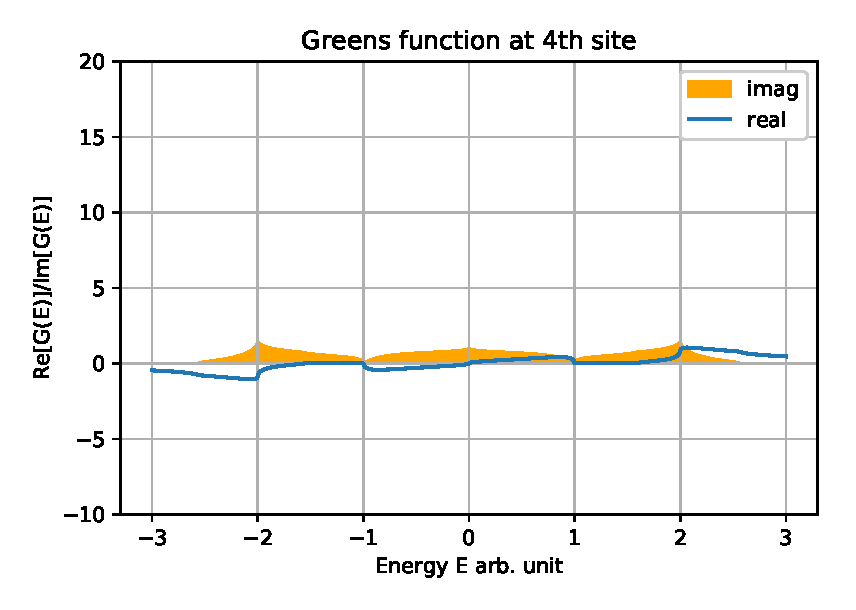
\includegraphics[width=\textwidth]{Figures/BetaimrealTE4.eps}
		\caption{Figure showing a plot of the Green's function at the 4th site}
		\label{4th}
	\end{subfigure}
	~ %add desired spacing between images, e. g. ~, \quad, \qquad, \hfill etc.
	%(or a blank line to force the subfigure onto a new line)
	\begin{subfigure}[b]{0.3\textwidth}
		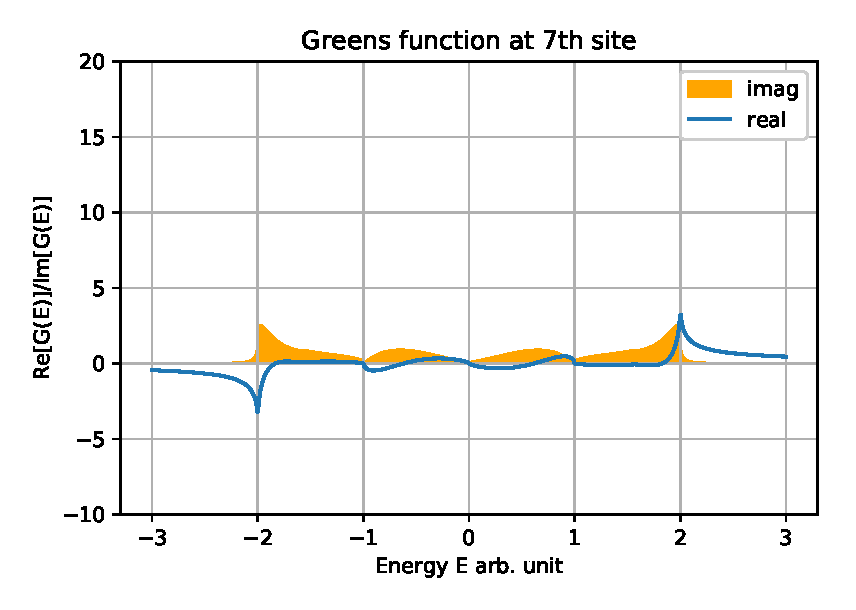
\includegraphics[width=\textwidth]{Figures/BetaimrealTE7.eps}
		\caption{Figure showing a plot of the Green's function at the 7th site}
		\label{7th}
	\end{subfigure}
	\caption{Two plots showing how the Green's function changes as the site is changed. The 4th and 7th sites are corresponding to atoms of those indices (4, 7) in \cref{pointplot}. Note how the LDOS changes (imaginary part) for the different sites.}\label{siteLDOSplot}
\end{figure}
\begin{figure}
	\centering
	\begin{subfigure}[b]{0.3\textwidth}
		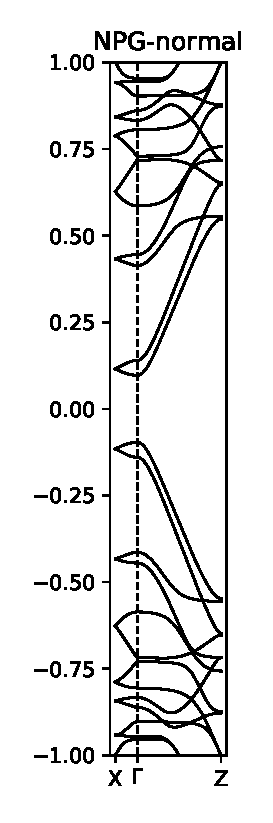
\includegraphics[width=\textwidth]{Figures/FabNPGBS.eps}
		\caption{Plot showing the band structure in the energy range \SI{-1.5}{\electronvolt} to \SI{1.5}{\electronvolt} for NPG with normal bridges between symmetry points \(X\) and \(Y\) with respect to \(\Gamma\)}
		\label{Fabbs}
	\end{subfigure}
	~ %add desired spacing between images, e. g. ~, \quad, \qquad, \hfill etc.
	%(or a blank line to force the subfigure onto a new line)
	\begin{subfigure}[b]{0.3\textwidth}
		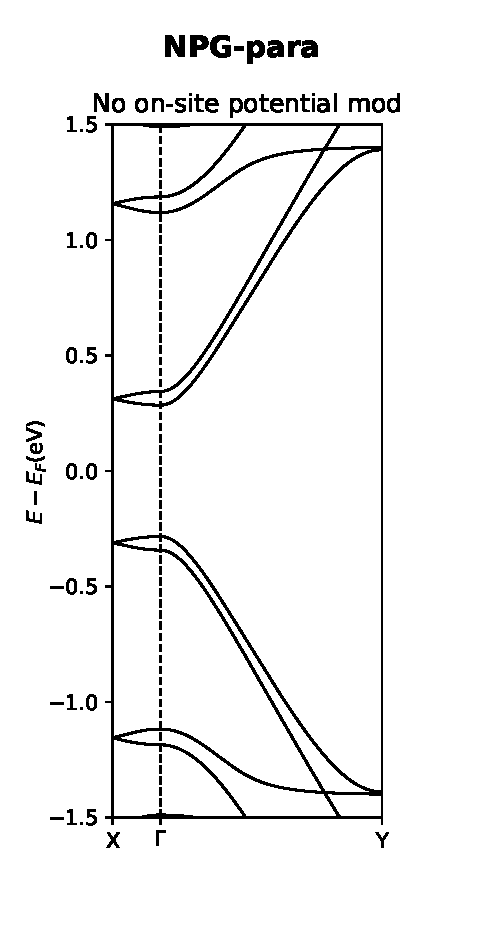
\includegraphics[width=\textwidth]{Figures/paraNPGBS.eps}
		\caption{Plot showing the band structure in the energy range \SI{-1.5}{\electronvolt} to \SI{1.5}{\electronvolt} for NPG with para bridges between symmetry points \(X\) and \(Y\) with respect to \(\Gamma\)}
		\label{parabs}
	\end{subfigure}
	~ %add desired spacing between images, e. g. ~, \quad, \qquad, \hfill etc.
	%(or a blank line to force the subfigure onto a new line)
	\begin{subfigure}[b]{0.3\textwidth}
		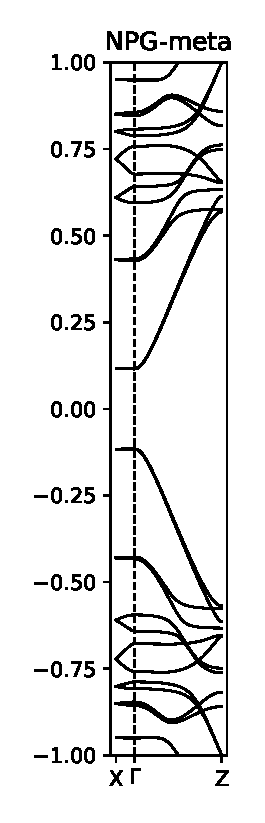
\includegraphics[width=\textwidth]{Figures/metaNPGBS.eps}
		\caption{Plot showing the band structure in the energy range \SI{-1.5}{\electronvolt} to \SI{1.5}{\electronvolt} for NPG with meta bridges between symmetry points \(X\) and \(Y\) with respect to \(\Gamma\)}
		\label{metabs}
	\end{subfigure}
	\caption{Figure showing para, meta and normal NPG band structures}\label{allbands}
\end{figure}
\im{Listings/Functions.py}{41}{47}
\vspace{-1\baselineskip}
\captionof{listing}{Function creating the hopping matrices between two sets of coordinates \label{hopfunc}}\vspace{\baselineskip}

\begin{figure}
	\centering
	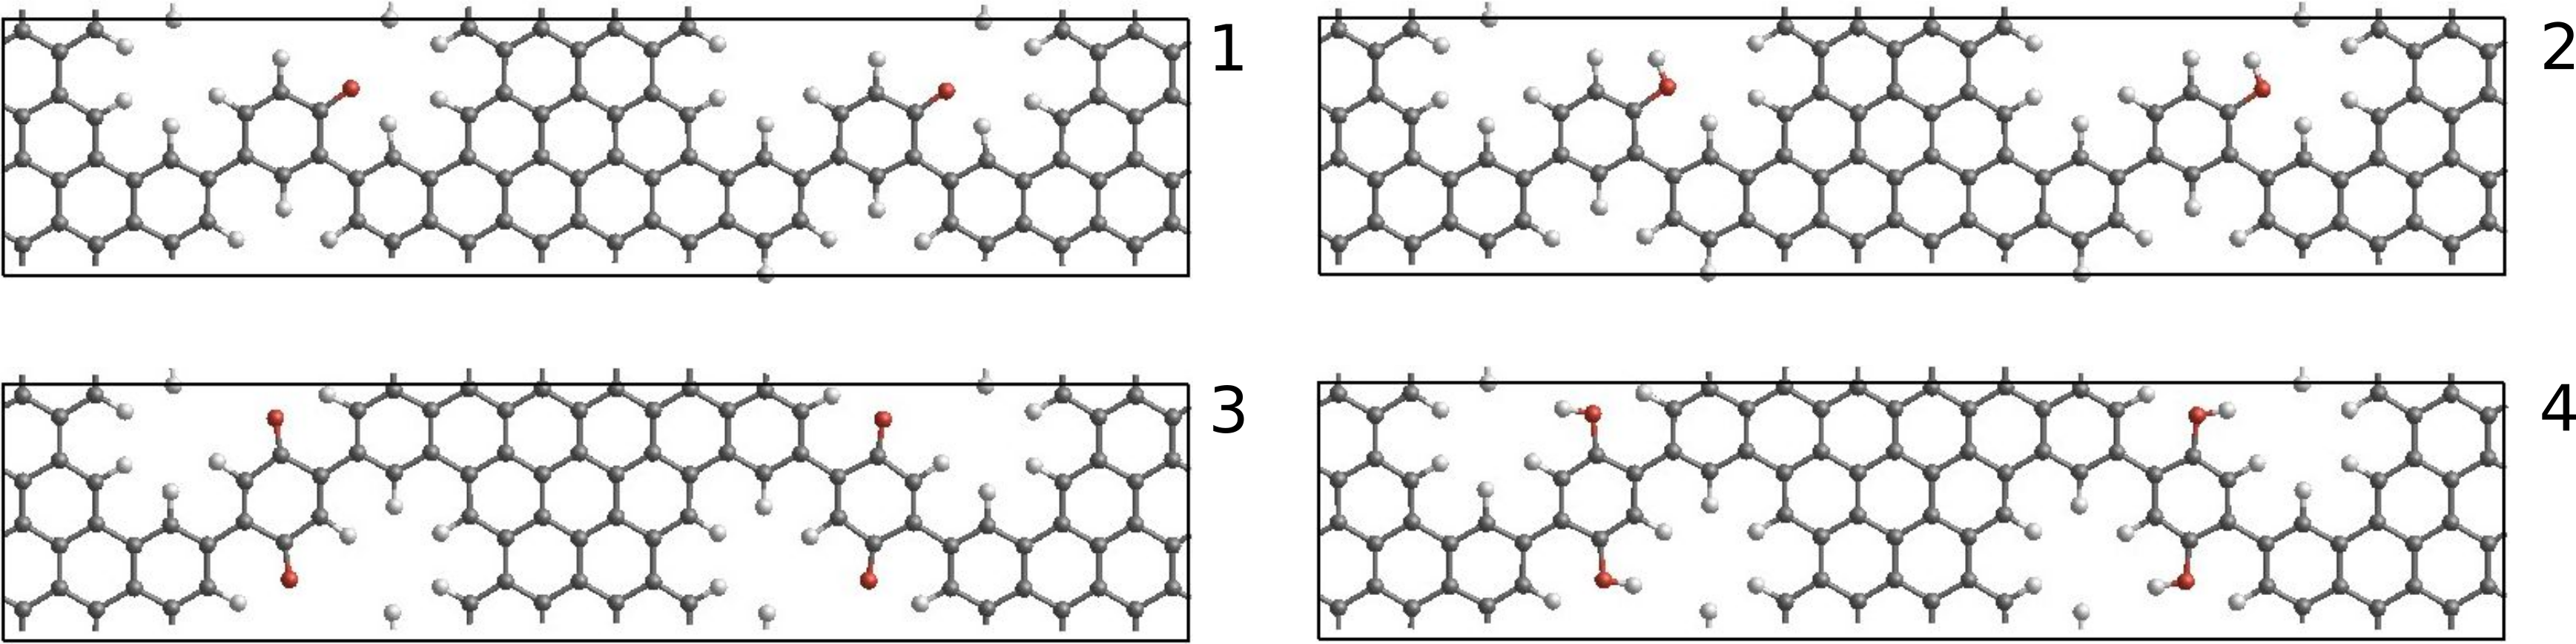
\includegraphics[width=\textwidth]{Figures/Structures.png}
	\caption{Figure showing all the structures stated in \cref{testtable}.}
	\label{Strucow}
\end{figure}

\im{Listings/Functions.py}{245}{252}
\vspace{-1\baselineskip}
\captionof{listing}{Code piece showing how the periodic Hamiltonian, shifted in the transverse direction i created using the given unit vector in the y direction.}{\label{periodichamilcode}}\vspace{\baselineskip}

\im{Listings/Functions.py}{234}{242}
\vspace{-1\baselineskip}
\captionof{listing}{Code piece showing how the transmission per energy point, using equation \cref{}.}{\label{transmissioncode}}\vspace{\baselineskip}

% \section{Project overview}
% A Gantt chart is provided on the next page. \textbf{Not Updated.}
% \newpage
% \begin{turnpage}
% \setcounter{myWeekNum}{6}
% \ganttset{%
% 	calendar week text={\myWeek{}}%
% }
% \begin{figure}\vspace{-10mm}
% \begin{ganttchart}[
% 		hgrid,
% 		vgrid={*{6}{draw=none}, dotted},
% 		x unit=.15cm,
% 		%	y unit title=.6cm,
% 		%	y unit chart=.6cm,
% 		inline,
% 		milestone inline label node/.append style={left=5mm},
% 		milestone/.append style={xscale=3},
% 		time slot format=isodate,
% 		time slot format/start date=2019-02-04
% 	]{2019-02-04}{2019-05-31}
% 	\gantttitlecalendar{year, month=shortname, week}\\
% 	\ganttgroup{Report writing}{2019-02-25}{2019-05-31}\\
% 	\ganttgroup[inline = false]{Course 33442}{2019-02-04}{2019-03-31}\\
% 	\ganttbar{Ch. 1 \& 2}{2019-02-04}{2019-02-17}\\
% 	\ganttlinkedbar[link bulge=2]{Ch. 3}{2019-02-18}{2019-02-24}\\
% 	\ganttlinkedbar[link bulge=2,bar inline label node/.style={right=15pt}]{Ch. 4 \& 5}{2019-02-25}{2019-03-03}\\
% 	\ganttgroup[inline = false]{Python code}{2019-03-04}{2019-03-31}\\
% 	\ganttbar{Py TB scripts}{2019-02-18}{2019-03-17}\\
% 	\ganttlinkedbar[link bulge=2, bar inline label node/.style={right=45pt}]{Small NPG systems simulations}{2019-03-10}{2019-03-31}\\
% 	\ganttmilestone{Proof of Concept with Python}{2019-03-31}\\
% 	\ganttgroup[inline = false]{Large scale TB}{2019-04-01}{2019-04-28}\\
% 	\ganttbar[bar inline label node/.style={left=10pt}]{SISL \& TBtrans tutorial}{2019-04-01}{2019-04-05}\\
% 	\ganttlinkedbar[link bulge=2, bar inline label node/.style={right=50pt}]{Setup NPG variations}{2019-04-06}{2019-04-28}\\
% 	\ganttgroup[inline = false]{Generate data}{2019-04-28}{2019-05-31}\\
% 	\ganttmilestone{Hand in report}{2019-05-31}
% \end{ganttchart}
% \end{figure}
% \end{turnpage}
% \clearpage
% \global\pdfpageattr\expandafter{\the\pdfpageattr/Rotate 90}

\end{document}
